\documentclass[12pt,a4paper]{article}
\usepackage[a4paper, margin=1in]{geometry}
\usepackage[utf8]{inputenc}
\usepackage[T1]{fontenc}
\usepackage{graphicx}
\usepackage{latexsym}
\usepackage{amsfonts,amssymb,amsmath,amsthm}
\usepackage{multirow}
\usepackage{multicol}
\setlength{\columnsep}{1.5cm}
\usepackage{setspace}
\usepackage{url}
\usepackage{array}
\usepackage{xfrac}
\usepackage{mwe}
\usepackage{tikz}
\usepackage{lmodern}
\usepackage{flowchart}
\usetikzlibrary{shapes,arrows,positioning,calc,fit}
\usepackage{graphics}
\usepackage{graphicx}
\usepackage{subfig}
\usepackage{booktabs}
\usepackage{float}
\usepackage{color,soul}
\usepackage{hyperref}
\usepackage{biblatex}
\addbibresource{References.bib}
\newcommand{\tom}[2]{{\color{red}{#1}}\footnote{\textit{\color{red}{#2}}}}
\newcommand{\ali}[2]{{\color{pink}{#1}}\footnote{\textit{\color{pink}{#2}}}}


\title{An Integral Projection Modeling Approach to Demographic Consequences of Multiple Partner Mutualisms}
\author{Ali M. Campbell\\
	Tom E.X. Miller}
\begin{document}
	\maketitle
	
	\section*{Abstract}
	
	Mutualisms are among the most widespread species interactions with diverse and dynamic consequences. They are considered more context dependent than other species interactions, meaning there are many different factors which influence the impacts of a mutualistic interaction, including partner diversity. Partner diversity has become a central focus in the field of mutualisms in recent years shifting the focus to multispecies mutualisms where the focus was previously on pairwise studies. It has been shown that pairwise studies are poor predictors of the effects of multispecies mutualistic interactions. The diversity of partners in a multi-species mutualism causes varied demographic effects on the population of the focal mutualist which can be explained by several mechanisms, portfolio effect, complementarity, and sampling effect. In this paper, I will focus on defensive ant-plant mutualisms. These involve plants which provide extra-floral nectar and/or “housing” to ants which in turn defend them from herbivores. While these interactions have been well studied in the literature, few have considered how diversity within partner guilds affect the overall benefits of mutualism for the plant partner. 
	I use the plant, Cylindropuntia imbracata (tree cholla), and ant, Crematogaster opuntiae (Crem.), Liometopum apiculatum (Liom.), and more, multispecies mutualism in which the cacti provide extrafloral nectar in exchange for defense from various herbivores and seed predators. I used 18 years of data collected from demographic censuses, which includes data such as size, survival, reproductive status, flowers produced, ant partner, and herbivory for 8 30x30 m plots, in New Mexico. With this data I parameterize a series of Bayesian generalized linear vital rate models to determine the impacts of different partners on the focal mutualists. I found that different ant partners did have different impacts on the vital rates of the tree cholla. Specifically, Crem. tended plants had advantages in both growth and survival when small, and Liom. tended plants had advantages in colonizing partners as well as floral viability. With these models I constructed an Integral Projection Model in which I could vary the presence of each partner, creating different “diversity scenarios”, to determine under which diversity scenario the focal mutualist experienced the highest fitness, and which of the above mechanisms may explain the effects of partner diversity in this system. I found that the real-life scenario (all possible ants are present) lead to the highest fitness for the tree cholla, indicating that partner diversity is beneficial in this system. It also shows that complementarity is at play in this system, meaning different partners offer different benefits leading to synergistic benefits for the tree cholla. 

\section*{Context/Introduction}

Mutualisms are species interactions in which all \tom{involved participants}{Notice the redundancy here. You don't need ``involved''.} benefit. They are among the most widespread species interactions\cite{Chamberlain2014, BoucherDouglasH.1985}, and are notoriously \tom{context dependent}{You need to define what you mean by this.} \cite{Bronstein1994,Chamberlain2014,Frederickson2013}, often deteriorating into other types of interactions, including parasitism \cite{Rodriguez-Rodriguez2017,Song2020,Mandyam2014,Thrall2007, Bahia2022}.
\tom{The benefits from these interactions are called rewards}{This is a pretty rudimentary definition, not necessary.}, but they require investment of resources or services into the interaction\cite{Bronstein2001}.
The presence of mutualists can shift the available \tom{habitat, fitness, or resource uptake}{These are very different things. I don't see why this sentence is needed in the context of your study.} of a partner\cite{Stachowicz2001,West2007}.
While mutualism is defined at the level of a species pair (+/+) these interactions are embedded in multi-species communities, such that a focal species (the focal mutualist) may engage with multiple partner species\cite{Stanton2013, Boucher1982}.\tom{}{I suggest you re-think whether most of this first paragraph is necessary.}

Partner diversity in mutualisms \tom{often leads to variable fitness benefits}{Not sure what you are saying here: different partners provide different fitness benefits? Or diversity per se has fitness benefits?} for the focal mutualist\cite{Afkhami2014, Palmer2010}, due to differences in partner quality\cite{Bascompte2019,Stanton2013,Frederickson2013,Jones2015, Ness2006}, differences in the types of benefits offered\cite{Kiers2003,Afkhami2014}, and direct interactions between partners\cite{Sun2019,Heath2009,Heath2014,Grutter2003}.
For these reasons, pairwise studies cannot be accurately used to predict the outcomes of \tom{multi-species mutualisms}{I think you need to operationally define this.}\cite{Palmer2010, Stanton2013, Chamberlain2014, Song2020}.
Studies on the effects of diverse multi-species mutualism systems are necessary to help us understand the demographic effects of partner diversity in mutualisms\cite{Bascompte2019}. 

Multi-species mutualism partner diversity causes varied demographic effects on the population of the focal mutualist which can be explained by a number of mechanisms.
Partners can vary in many ways: in some cases, the quality varies leading to some true mutualist partners, \tom{some freeloaders, and even some parasites}{What is the difference between a freeloader and a parasite?} \cite{Bronstein1994,Bronstein2001a,Afkhami2014,Song2020,West2007,Frederickson2013,Jones2015}; in other cases, \tom{the function of the partner can vary}{I think I know what you mean but you should clarify for other readers what is the difference between quality and function.}, each offering a different type of reward to the focal mutualist \cite{Stanton2003}.
\tom{When there is a consistent partner hierarchy based on benefits offered, a more diverse sample of the partner community may be more likely to include the highest quality partner (the one which offers the focal mutualist the most benefit)\cite{Frederickson2013}.}{I think the content of this paragraph needs to be better organized. Describing ways in which partner species differ is conceptually very different than describing mechanisms by which partner diversity can be beneficial -- yet this paragraph seems to glom them together. The ``partners are different'' content seems to fit better in the previous paragraph.}
When the fitness of a focal mutualist with multiple partners is equal to the fitness of a focal mutualist with only the highest quality partner, as shown in \tom{Figure}{This figure is great for talks but I don't recommend it for a publication.} \ref{fig:comp-samp}b, sampling effect can explain \tom{the positive effects}{When you say \emph{the} positive effects of partner diversity, does that imply that diversity effects are always positive? I think this is the first you've said that partner diversity is beneficial.} of partner diversity\cite{Batstone2018}. 
Partners can also vary functionally, meaning each partner offers a different type of reward to the focal mutualist\cite{Stachowicz2005,Bronstein2006,Stanton2003}.
When this leads to a higher fitness for the focal mutualist than any single interaction,as shown in Figure \ref{fig:comp-samp}a, complementarity explains the benefits of partner diversity\cite{Batstone2018}. 
Partners can also have asynchronous responses to the environment, either spatially\cite{Ollerton2006} or temporally\cite{Alarcon2008}.
Multiple partners can act as a 'portfolio' leading to more even fitness benefits across environmental or temporal heterogeneity, as shown in Figure \ref{fig:portfolio}, through the portfolio effect\cite{Batstone2018,Lazaro2022}.

\begin{figure}[h]
	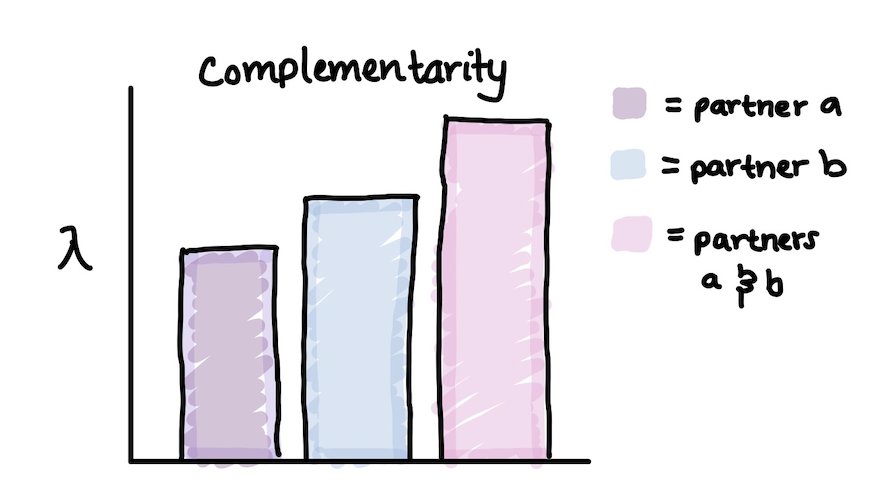
\includegraphics[width=0.58\linewidth]{complementarity.png}
	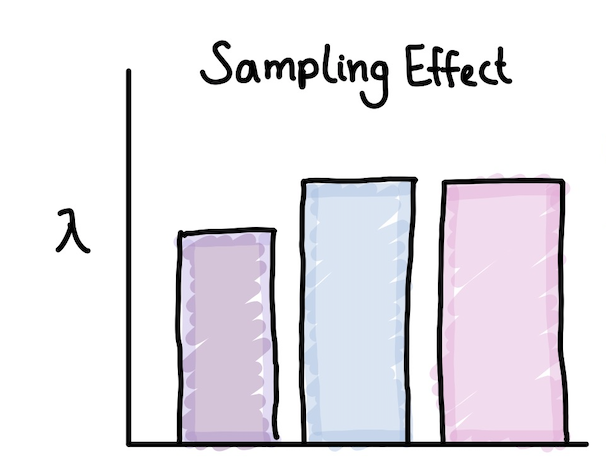
\includegraphics[width=0.40\linewidth]{sampling_effect.png}
	\caption{asdasdf}
	\label{fig:comp-samp}
\end{figure}
\begin{figure}[h]
	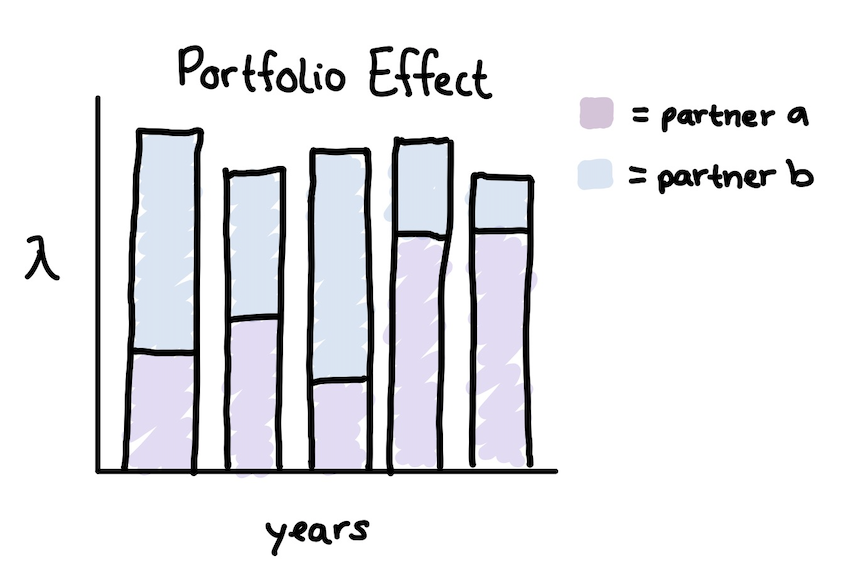
\includegraphics[width=0.60\linewidth]{portfolio_effect.png}
	\caption{asdasdf}
	\label{fig:portfolio}
\end{figure}


When multiple partners are present, \tom{partner turnover}{I suggest introducing this idea a little differently. Partner diversity can have different effects depending on whether it manifests all at once or sequentially. So this leads to the question of turnover.} is also important to consider, \tom{as partner identity has been shown to impact benefits in mutualisms}{You have made this point several times.}\cite{Djieto-Lordon2005, Ness2006, Bruna2014}. 
Turnover can happen at different timescales\cite{Oliveira1999,Horvitz1986} from minutes to years. 
The degree and order of partner turnover can have important impacts on the fitness of the focal mutualist.
High degrees of partner turnover, \tom{also known as opportunism}{I've never seen partner turnover referred to as ``opportunism''.}, may offer \tom{buffering in the face of environmental variation}{This sounds a lot like portfolio effect, so I think you need to clarify how it relates.}\cite{Hegland2009}, while low degrees of partner turnover, also known as partner fidelity, \tom{can increase the benefits}{This makes it sounds like diversity is harmful - since low turnover means low diversity. Is that an example of negative effects of partner diversity?} received in a mutualism\cite{Sachs2004}.
\tom{The direction of turnover can also have a significant impact, particularly if the most beneficial partner changes across the ontogeny of the focal mutualist's life\cite{Fonseca2003}.
For example, susceptibility to enemies can change across life stages\cite{Boege2005,Barton2010}, so can defense traits, indicating that the focal mutualist benefits the most when defensive partners align with focal mutualist development\cite{Djieto-Lordon2005}.}{This is an excellent point. The second sentence here is a little clunky - see if you can fine-tune it.} 

\tom{Defensive}{Better transition from concepts to ants?} ant-plant mutualisms are common interactions in which plants provide \tom{extra-floral nectar}{I would just say ``food'' -- see Beltian bodies as another food resource} and/or ``housing'' to ants which in turn defend them from herbivores\cite{Bronstein1998, Bronstein2006}. 
\tom{Ants are highly ubiquitous\cite{Schultheiss2022} and vary significantly in abundances\cite{Schultheiss2022}}{This seems like too general/vague a statement to be useful here.}, types of rewards offered\cite{Beattie1985}, and \tom{quality of interaction}{What do you mean by this and how does it differ from types of rewards?} with their plant partners\cite{Rico-Gray1989,Palmer2010}, \tom{making these interactions great systems to study the effects of partner diversity}{A simpler and more to-the-point observation is that these interactions are typically generalized: most EFN plants have multiple ant partners} within mutualisms. 
\tom{While these interactions have been well studied\cite{Ness2006,Beattie1985,Schultheiss2022} \st{in the literature}, few have considered how diversity within ant defender guilds\cite{Stanton2013} or temporal fluctuations in partner interactions\cite{Trøjelsgaard2015} affect the overall benefits of mutualism for the plant partner.}{Good sentence.} 

This study focuses on the tree cholla cactus, a long lived \textit{Cylindriopuntia imbricata}, \st{long-lived} EFN-bearing plant that associates with multiple species of ant partners.
Insect herbivory negatively affects the growth of cacti, in turn reducing population growth rates\cite{Miller2009}. 
\st{The} ant partners defend the cacti from these insect herbivores, reducing the negative effects of herbivory\cite{Miller2007}. 
The multiple ant partners do not co-occur on \tom{individual}{} plants, but a single cactus may interact with multiple species over its lifetime.
Some of the ant partners are more effective defenders than others, with \tom{\textit{Liom.}}{Notice that you have not yet introduced the species, let alone the abbreviation of its latin name, so a reader will be very confused here. Try to anticipate what your readers need to stay with you.} tended reproducing plants experiencing the lowest level of herbivory as shown in \tom{Figure \ref{fig:herb}}{You have put a result in the Introduction. Sometimes this is appropriate but I don't think it is here. You have not described any methods for where this result comes from, so it is not reproducible. Make this a result.}.
\tom{This shows that although all the ants associated with the tree cholla are within one guild, they are not all equal and may have different demographic effects on the cacti.}{I think you can make this point without needing the figure, based on what we have already published from this system. It is also worth pointig out that one of the defenders was suggested to be net-negative because it deterred pollinators (Ohm and Miller 2014) but that study did not integrate demographic effects over the life cycle, which is what you do here and worth emphasizing as a source of novelty.}

\begin{figure}[h]
	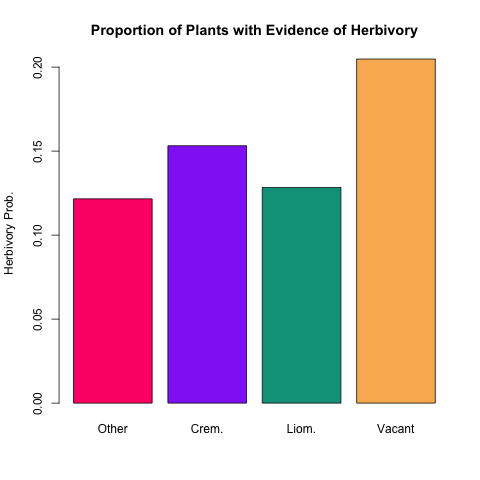
\includegraphics[width=.8\linewidth]{herb_ant_only_flow.png}
	\caption{asdasdf}
	\label{fig:herb}
\end{figure}

In this \tom{paper}{Refer to this as a study and not a paper.} we will answer three questions about the demographic effects of partner diversity in multi-species mutualisms:
\begin{enumerate}
	\item{What are the contrasting demographic effects of multiple partners?}
	\item{How do \tom{size}{size of what?} and partner identity impact the directionality of turnover between multiple partners?}
	\item{\tom{What mechanisms explain the benefits}{This question pre-supposes that there are benefits of diversity.} of partner diversity in a multispecies mutualism?}
\end{enumerate}


\tom{To answer these questions, we used a long-term dataset of demographic information (size, survival, number of flowers produced or aborted, etc.) and ant partner data (species, number of ants) to track the structure of the population across time as well as individual level impacts of ant partners on the cacti.}{I think this sentence can be sharpened. I don't think that details like flower abortion and ant number are important to include here, but I also don't think this sentence really communicates the nature or volume of the data,} 
We analyzed the \tom{impacts of partner diversity}{The vital rate models do not reflect the impact of partner diversity, they are simply vital rate estimates fit with ant category as a factor -- be careful with how you present this.} on each individual vital rate (survival, growth, floral viability, etc.) with \tom{Bayesian models}{``Bayesian models'' does not carry much meaning. A model cannot be intrinsically Bayesian. The model is the model, and Bayesian analysis is one way to estimate it's parameters.}, which we used to parameterize an Integral Projection Model (IPM).
In previous studies the effects of multiple partners, and the dynamics of their turnovers, have been identified and quantified\cite{Palmer2010, Nishi2013, Hussa2013}, but \tom{none have identified the mechanisms that explain the benefits of partner diversity}{Not sure I agree here. How are you ``identifying mechanisms'' in a way that Palmer et al. did not, for example?}. 


\section*{Methods}
\subsection*{Study System}

\st{To determine how interactions with multiple partners impacts the cacti over time, we have monitored a population of tree cholla annually since 2004.} 
This study was conducted in the Los \tom{Pinos}{there is an accent on the n} mountains, a small mountain chain located on the Sevilleta National Wildlife Refuge, a Long-term Ecological Research (LTER) site in central New Mexico \tom{(34*20’5.3’’N, 106*37’53.2’’W)}{I would not give lat-long here. We should provied lat-long of each plot as part of the full data that we make available.}.
This is an area characterized by steep, rocky slopes, and perennial vegetation like cacti and junipers. 
\st{The} tree cholla cacti are common in high Chihuahuan desert habitats, with their native range spanning the southwestern USA\cite{Benson1982}. 
These arborescent cacti produce cylindrical segments with large spines. 
In the growing season, May to August in New Mexico, the plants initiate new vegetative segments and flower buds at the ends of existing segments. 
While most plants produce new segments every season, only those which are reproductively mature produce flower buds. 
Tree cholla generally reach at least 9 years of age before beginning to reproduce *** I found this being cited as unpublished data in Ohm Miller 2014 ***. 
Like other EFN-bearing cacti, tree cholla cacti secrete nectar from specialized glands on young vegetative and reproductive structures\cite{Ness2006,Oliveira1999}.

This EFN is harvested by various ant species in return for defense. 
At the Sevilleta, the cacti are visited primarily by two species of ground-nesting ants from the formicoid clade, \textit{Crematogaster opuntiae (Crem.) } and \textit{Liometopum apiculatum \tom{(Liom.)}{I know I have used these abbreviations in previous papers but I would not recommend doing so again. More professional and appropriate to refer to \emph{L. apiculatum}, etc.}, } as well as other rarer species, including \textit{Forelius pruinosus (For.) }, a \tom{\textit{Phenogaster}}{Incorrect spelling.} \tom{ant}{Obviously it's an ant.}, and \textit{Camponotus spp. (Camp.)}.

\begin{figure}[h]
	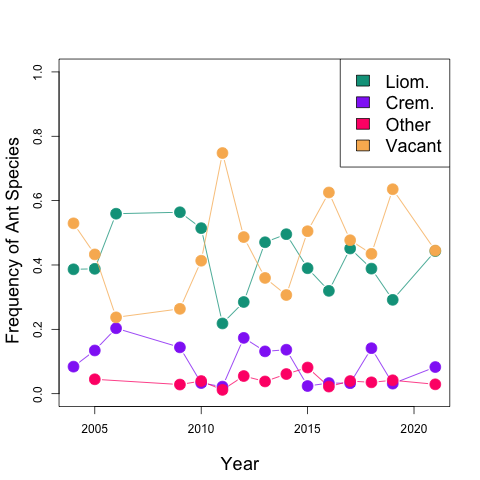
\includegraphics[width=\linewidth]{Timeseries.png}
	\caption{asdfasdfsadfasdf}
	\label{fig:timeseries}
\end{figure}


\textit{Liom.} ants were the most frequent visitors, present a  between 25\% - 60\% of cacti \tom{annually}{Unclear what you mean by ``annually''? Think about the most technically correct and most efficient way to communicate these results.}, \textit{Crem.} were present at between 0\% - 20\% of cacti, and \textit{For.} were present at between 0\% - 5\% of cacti in any given year, as shown in \tom{Figure}{Again, you have slipped in a result without providing any methods. There is a similar figure in Donald and Miller 2022, so you can cite that paper when you report frequencies of association.} \ref{fig:timeseries}. 
\tom{\st{It is important to note that not all cacti are visited every season, they can remain vacant, in fact} }{Notice that this part of the sentence does not provide any information that is not in the second part.}up to 80\% of cacti are vacant in any given year. 

These ants rarely co-occur on a plant, probably due to interspecific competition\cite{Miller2007}\tom{, rather}{Grammatically awkward. I would start a new sentence Instead, each cactus} each cactus is visited by a single ant species for the duration of a season, and the \tom{visitor}{What do you mean by visitor? Is each individual ant a visitor?} can change from one season to the next. 
\tom{Across the entire lifespan cacti may interact with multiple species of partners. }{This is implied by the sentences above so there is no new information here.}
At the beginning of the growing season, when EFN production begins, the ground-nesting ants will begin visiting tree cholla.
They will visit the cacti every day during the season from early morning *** to sunset *** \tom{abandoning the cacti at night for their nests}{Incorrect. See Ohm and Miller 2014.}. 
In late August, the tree cholla will stop producing EFN and the ants will stop visiting until the next growing season. 
\tom{The process by which ants are sorted out onto different cacti is somewhat of a mystery}{too colloquial}, but we know several facts which likely influence the process. 
Smaller cacti are less likely to be visited because they produce very little EFN, so larger cacti are generally more desirable\cite{Miller2014}. 
Similarly, many factors go into how many vegetative segments and floral buds are produced in a particular growing season, so the more productive cacti are also more \tom{desirable}{I don't yhink we should speculate about ants' desires.}. 
Some of the ant species are considered more aggressive, specifically \textit{Liom.}\cite{Miller2007}, which may be advantageous in \tom{going after}{too colloquial} more desirable cacti. 
Some ants are also more likely to retain the same tree cholla partners year after year, meaning they reduce the partner turnover experienced by individual cacti. 
These factors mean that by some hierarchy at the beginning of the season the ants claim a subset of the existing cacti and visit them regularly throughout the season, and that from season to season the same ant species may visit the same cacti, but it is not guaranteed. 
\ali{Note.}{I am not sure how much of this I should include here, since some of the turnover info is results from this paper?}\tom{}{Yes this is what I was thinnking as i was reading. Much of this fall out of the results of your analysis. I would significantly reduce this paragraph. Think about what your readers need to know to process what's to come.}
\st{These ants defend the tree cholla from various seed predators and herbivores in exchange for the EFN.} 

There are a variety of insect herbivores and seed predators which attack the cacti, focusing either on the vegetative segments and the reproductive segments \tom{throughout the entire range}{range info not really pertinent} of the tree cholla\cite{Mann1969}. 
\tom{More locally, at the Sevilleta, there are several insects which occur commonly on these cacti.
These include an unidentified weevil, a cactus bug, and a seed predator. }{Notice how these sentences add no information to the paragraph.}
The unidentified weevil of the genus \textit{Gerstaekeria} which feed on vegetative and reproductive structures and implant their larvae within the plant for the winter. 
The cactus bug, \textit{Narnia pallidicornis}, (Hemiptera: Coreidae) feed on all cactus parts with a preference for the reproductive structures \cite{Miller2006}.
The seed predator, \textit{Cahela ponderosella}, (Lepidoptera: Pyralidae) attack developing fruits pre-dispersal and oviposit in open flowers mid-growing season where larvae burrow into the ripening ovary. 
These predators can have significant negative impacts on the fitness of individual cacti and depress population growth\cite{Miller2009}.\tom{}{I think it is also important to summarize what is known about ant defense against these insects from previous papers. The fact that we have experimental evidence that ants provide defense is important to include, because your data are all observational.} 

\tom{\section*{Methods}}{Some duplication here...?}
\subsection*{Study System}
\subsection*{Natural History}
To determine how interactions with multiple partners impacts the cacti over time, we have monitored a population of tree cholla annually since 2004. 
This study was conducted in the Los Pinos mountains, a small mountain chain located on the Sevilleta National Wildlife Refuge, a Long-term Ecological Research (LTER) site in central New Mexico (34*20’5.3’’N, 106*37’53.2’’W).
This is an area characterized by steep, rocky slopes, perennial vegetation like cacti and junipers. 
The tree cholla cacti are common in high Chihuahuan desert habitats, with their native range spanning the southwestern USA\cite{Benson1982}. 
These arborescent cacti produce cylindrical segments with large spines. 
In the growing season, May to August in New Mexico, the plants initiate new vegetative segments and flower buds at the ends of existing segments. 
While most plants produce new segments every season, only those which are mature enough produce flower buds. 
Tree cholla generally reach at least 9 years of age before beginning to reproduce *** I found this being cited as unpublished data in Ohm Miller 2014 ***. 
Like other EFN-bearing cacti, tree cholla cacti secrete nectar from specialized glands on young vegetative or reproductive structures\cite{Ness2006,Oliveira1999}.

This EFN is harvested by various ant species in return for defense. 
At the Sevilleta, the cacti are visited primarily by two species of ground-nesting ants from the formicoid clade, \textit{Crematogaster opuntiae (Crem.) } and \textit{Liometopum apiculatum (Liom.), } as well as other rarer species, including \textit{Forelius pruinosus (For.) } and \textit{Camponotus spp. (Camp.)}.

\textit{Liom.} ants were the most frequent visitors, present a  between 25\% - 60\% of cacti annually, \textit{Crem.} were present at between 0\% - 20\% of cacti, and \textit{For.} were present at between 0\% - 5\% of cacti in any given year \ref{Fig:Ant_freq}. 
It is important to note that not all cacti are visited every season, they can remain vacant, in fact up to 80\% of cacti are vacant in any given year. 

These ants rarely co-occur on a plant, probably due to interspecific competition\cite{Miller2007}, rather each cactus is visited by a single ant species for the duration of a season, and the visitor can change from one season to the next. 
Across the entire lifespan cacti may interact with multiple species of partners. 
At the beginning of the growing season, when EFN production begins, the ground-nesting ants will begin visiting tree cholla.
They will visit the cacti every day during the season from early morning *** to sunset *** abandoning the cacti at night for their nests. 
In late August, the tree cholla will stop producing EFN and the ants will stop visiting until the next growing season. 
The process by which ants are sorted out onto different cacti is somewhat of a mystery, but we know several facts which likely influence the process. 
Smaller cacti are less likely to be visited because they produce very little EFN, so larger cacti are generally more desirable\cite{Miller2014}. 
Similarly, many factors go into how many vegetative segments and floral buds are produced in a particular growing season, so the more productive cacti are also more desirable. 
Some of the ant species are considered more aggressive, specifically \textit{Liom.}\cite{Miller2007}, which may be advantageous in going after more desirable cacti. 
Some ants are also more likely to retain the same tree cholla partners year after year, meaning they reduce the partner turnover experienced by individual cacti. 
These factors mean that by some hierarchy at the beginning of the season the ants claim a subset of the existing cacti and visit them regularly throughout the season, and that from season to season the same ant species may visit the same cacti, but it is not guaranteed. 
\ali{Note.}{I am not sure how much of this I should include here, since some of the turnover info is results from this paper?}
These ants defend the tree cholla from various seed predators and herbivores in exchange for the EFN. 

There are a variety of insect herbivores and seed predators which attack the cacti, focusing either on the vegetative segments and the reproductive segments throughout the entire range of the tree cholla\cite{Mann1969}. 
More locally, at the Sevilleta, there are several insects which occur commonly on these cacti.
These include an unidentified weevil, a cactus bug, and a seed predator. 
The unidentified weevil of the genus \textit{Gerstaekeria} which feed on vegetative and reproductive structures and implant their larvae within the plant for the winter. 
The cactus bug, \textit{Narnia pallidicornis}, (Hemiptera: Coreidae) feed on all cactus parts with a preference for the reproductive structures \cite{Miller2006}.
The seed predator, \textit{Cahela ponderosella}, (Lepidoptera: Pyralidae) attack developing fruits pre-dispersal and oviposit in open flowers mid-growing season where larvae burrow into the ripening ovary. 
These predators can have significant negative impacts on the fitness of individual cacti and depress population growth\cite{Miller 2009}. 
	
	\subsection*{Data}
	
	The data collected \tom{on these cacti}{notice how these words add nothing} are from a long-term dataset spanning 2004 to 2022 taken from our eight 30 $\times$ 30 meter plots at the Sevilleta LTER. 
	\tom{The data initially included 134 naturally occurring plants across 4 spatial blocks censused annually from 2004 to 2008.}{this seems to contradict what you just said about eight plots.}
	Six of the 30 $\times$ 30 meter plots \tom{were created with naturally occurring plants}{this sounds funny, meaning unclear}, censused from 2009 to \tom{2014}{Not sure why you have these ending in 2014. These are plots 1-6, which we continue to collect data from}. 
	The final two plots were added to this census from 2011 onwards. 
	The distribution of these eight plots are shown in \tom{figure}{you probably don't need a plot map - maybe in the supplement} \ref{fig:map}.
		Annually, in May we surveyed these plots, taking many types of demographic and partner data. 
		For each plant, we recorded the height (cm), maximum crown width, and \st{perpendicular }crown width perpendicular to the maximum, which are used to calculate plant volume (\tom{cm3}{make this a superscript}) based on the volume of a cone with the mean of maximum crown width and perpendicular crown width as the diameter. 
		We recorded plant \tom{survival}{I would start with survival because if it's dead nothing else is recorded} from the last survey to the current survey\st{ as a binary data point, 0 (died) or 1 (survived)}. 
		We recorded the total number of flower buds, including how many were aborted and how many were not\st{, which we used to calculate the viability rates of the cacti}. 
		We recorded all ant species present, usually just one, and the number of ants we could count in 30 seconds. 
		We also recorded the species of herbivore or \tom{seed predator}{we do not record seed predator data}, the number present on the plant, and \tom{if there is any clear, new evidence of herbivory}{beware that this has not been very consistent} on the tree cholla segments. 
		
		In addition to this primary dataset, I used \tom{several other datasets}{I don't think you need to say much here, you can cite prevous papers when you describe these parts of the IPM} throughout the analysis in this paper.  Look at how Tom has described these. Cite these other papers which this data comes from. 
		The second dataset was *** germination rates.
		The third dataset was *** pre-census survival.
		The fourth dataset was *** $JO_fruit_data_final_dropplant0.csv$.
		
		\subsection*{Demographic Modeling}
		
		The \tom{statistical models described above}{they are actually below - but i would put them above.} parameterize the Integral Projection Model (IPM) that we used to estimate population growth under various partner conditions.  
		IPMs are used to estimate fitness of a population across a \tom{continuous variable}{you actually have both continuous and discrete variables}, \tom{rather than using a stage- or size-specific variable}{not an accurate description of how IPMs differ from MPMs} to categorize the population. 
		This IPM was used to estimate the \tom{growth rate }{not just growth rate, but growthrate as a function of partner identity and diversity -- important to include}of the tree cholla population, \tom{effectively}{why effectively?} a quantitative measure of the fitness of the population. 
		
		Following previous studies, we modeled the life cycle of \tom{\textit{C. imbricata}}{sometimes you say cholla, sometimes cacti, sometimes the latin name -- stay consistent} using continuously size-structured plants,\tom{$n_i(x)$}{what is n? what is i? what is x?}, and two discrete \tom{seed banks}{there is no beta in the model below. what is t?} ($\beta_{1,t}$ and $\beta_{2,t}$) corresponding to 1 and 2-year old seeds.
		$$
		B_{1, t+1} = \kappa \delta \sum_{i}^{4} \int_L^U P(x) A_i(x) F(x)n_i(x) dx \\
		$$
		$$
		B_{2,t+1} =  (1 - \gamma_1)B_{1,t}\\
		$$
		
		The functions $P$, $F$, and $A$ give the probability of flowering, the number of flowerbuds produced, and the proportion of flowerbuds which will create seeds. 
		Each of these functions, \st{estimated by a Bayesian model} \tom{calculates}{the function does not do any calculation} these values for an $x$-sized plant in year $t$. 
		The proportion of flowerbuds which will produce seeds ($A$) is also dependent on the ant species present on the plant $i$ in year $t$. 
		The integral is multiplied by the number of seeds per fruit ($\kappa$) and the probability of seed dispersal/survival ($\delta$) to give the number of seeds that enter the 1-year old seed bank. 
		Parameters $U$ and $L$ are the upper and lower bounds, respectively, of the plant size distribution. 
		Plants can recruit out of the 1-year seed bank with the probability of $\gamma_1$ or transition to the 2-year seed bank with a probability of $1 - \gamma_1$. 
		Seeds in the 2-year seed bank are assumed to either germinate with a probability of $\gamma_2$ or die. 
		
		The size dynamics of the plants are given by:
		
		$$
		n(y,i)_{t+1} = (\gamma_1 B_{1,t} + \gamma_2 B_{2,t}) \eta(y) \omega \beta_i  + \\
		$$
		$$
		\sum_{j}^{4} \int_L^U S_j(x) G_j(y,x) \tau_{ij}(x) n_j(x) dx \\
		$$
		
		The final equation gives the \tom{stochastic population composition }{what does this mean?}in terms of size and ant state of the \textit{C. imbracata} population $n$ in year $t+1$ based on the vital rates and size $n$ of the population in year $t$.
		The first term gives the recruitment from 1 and 2-year seedbanks to size $y$.
		$\eta(y)$ gives the seedling size distribution, which is assumed to be normally distributed, and $\omega$ gives the proportion of seedlings which survive from germination (late summer) to the census (May). 
		The second term gives the changes in the population of the cacti which are not recruits. 
		The functions $S$ and $G$ give the probabilities of surviving from year $t$ to $t+1$ and growing to size $y$ from year $t$ to year $t+1$, respectively. 
		Each depends on the size $x$ in year $t$ and the ant state $j$ in year $t+1$. 
		Finally, $\tau_{ij}$ is the probability of a cactus which is size $x$ with ant partner $i$ in year $t$ being tended by ant partner $j$ in year $t+1$.\tom{}{the ants dynamics of the model need to be presented more thoroughly and clearly.} 
		
		\tom{}{This paragraph should get its own subsection. This is about model analysis, not model structure.}\tom{Because many of the vital rates were ant-specific}{you need to explain why some are and some are not}, we were able to consider the composition of the population with the presence of any single ant species, or any combination of ant species (with vacancy always included).
		These options include: complete vacancy; \textit{Liom.} and vacancy; \textit{Crem.} and vacancy; other and vacancy; \textit{Liom.}, \textit{Crem.}, and vacancy, \textit{Liom.}, other, and vacancy; \textit{Crem.}, other, and vacancy; and all ant partners and vacancy.
		We used this option to calculate the distribution of stochastic population fitness for each combination of ant partners to determine if there is benefit from partner diversity and if there is an optimal combination of partners for this system. 
		We then used these fitnesses and \tom{the yearly break-downs of the model}{what does this mean?} to determine if there was \tom{evidence of any biodiversity ecosystem function mechanisms to explain any partner diversity benefits}{you never describe any criteria for detecting the different mechanisms. What does one need to see in data to conclude that one or another is operating?}. 
		
		\subsection*{Statistical Modeling}
		At the start of this section say for all models unless otherwise noted we used vague priors. 
		Also need to introduce the names of these functions ex: survival = s(x)
		With the primary dataset above we fit a series of generalized linear mixed models (GLMMs) in a hierarchical Bayesian framework, meaning the output is a distribution of \tom{the interaction between various factors on the highlighted variable}{confusing} rather than a maximum likelihood estimate with both fixed and random effects, which predicts the probability of a given process based on the size of the cacti, the presence of different ant partners, the year, and the plot.\tom{}{this is a confusing sentence. try to sharpen this.}
		Unless otherwise mentioned, all models used vague priors. 
		The growth model ($G_j(y,x)$) estimated the \tom{growth rate}{this is not what you modeled} of cacti, with fixed effects for the size and ant partner and random effects for plot and year, using a Normal distribution, with standard deviation dependent on the size of the cactus \tom{also with a Normal distribution}{??}. 
		The survival model ($S_j(x)$) estimated the probability of survival, with fixed effects for the size of the cactus and ant partner and random effects for plot and year, using a Bernoulli distribution. 
		The reproduction model ($P(x)$) estimated the probability of reproducing each year, with fixed effects for the size of the cactus and random effects for plot and year, using a Bernoulli distribution. 
		The total flowers model ($F(x)$) estimated the total flowers produced by a plant, with fixed effects for its size and random effects for plot and year, using a \tom{Truncated}{truncated how?} Negative Binomial distribution. 
		The viability model ($A_i(x)$) estimated the proportion of flowers produced by a plant which are viable (not aborted), with fixed effects for the size of the cactus and the \tom{presence of ant partners}{this is not the variable in the model} and random effects for plot and year, using a Binomial distribution.
		The ant transition rates model ($\tau_{i,j}(x)$) estimates the probability of a cactus being visited by an ant partner, with fixed effects for the size of the cactus and the previous ant partner and random effects for plot and year, using a Multinomial distribution.  
		The recruit size model ($n_j(x)$) estimates the size distribution of all recruits from a year, with no fixed or random effects, using a Normal distribution. 
		With the \tom{second dataset}{what second data set? same question for 3 and 4} above, we fit a two Bayesian generalized linear models for the 
		probability of germinating from a seed in the first year ($\gamma_1$) or the second year ($1 - \gamma_1$) using a Binomial distribution.
		With the third dataset above, we fit a Bayesian generalized linear model for the probability of a seedling, which has sprouted each year, surviving to May ($\delta$) when we visit (accounting for missed mortality events), with fixed effects for the previous size and transect random effects, using a Bernoulli distribution. 
		With the fourth dataset above, we fit a Bayesian generalized linear model for the number of seeds produced by every flower on a cactus ($\kappa$) based on the ant partner, using a Negative Binomial distribution. 
		
		These Bayesian GLMMs were run with STAN through version 4.0.2  of R using \tom{1000 iterations}{do you mean 10000? 1000 is not very many}, \tom{150 warmups, 3 chains, and 1 thins.}{``warmups'' and ``thins'' are not the right word choices} 
		To assess the convergence of our models we checked the trace of each mcmc chain (the convergence graphs are shown in the supplemental documents in Figures ***).
		To assess the fit we simulated data from the models and compared this to the real data (the fit plots are shown in the supplemental documents in Figures ***).
		
		\tom{With these models, we investigated the impacts of different ant species on the processes of vital rates and the probabilities of individual cacti interacting with each ant species.
		To address our first goal, we compared the effects of ant partners on the growth rate, survival rate, and the viability of flowers across sizes. 
		We also broke these effects down by every year of data to see if the impacts of ant partners varied across years. 
		To address the second goal, we compared the probability of being visited by a given ant based on each possible previous partner to note any patterns of ant tending. 
		We also broke these interactions down by every year of data to see if the patterns changed across years. }{This needs a much more thorough explanation. You have not described any methods for a stochastic analysis. You need a new section here explaining these methods in a way that is reproducible. Keep in mind that reproducibility is the standard we are aiming for, and in the current draft, just about all of the methods fall short of that standard.}
		
		\vspace{1cm}
		
		
		\section*{Results}
		\tom{I’m honestly not sure what all should be included here. I feel like I need a lot more info about the specifics???}{Let's talk about this.}
		
		\subsection*{Vital Rates}
		\begin{figure}[h]
			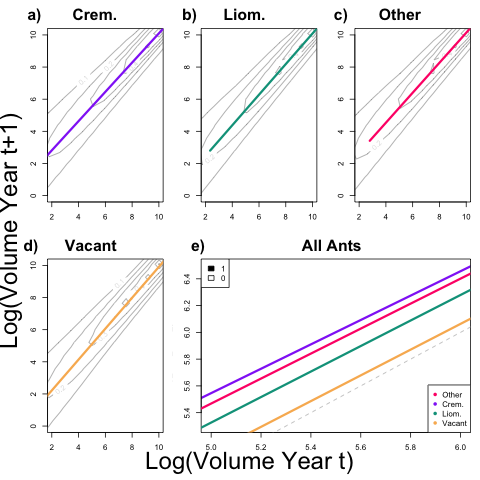
\includegraphics[width=0.58\linewidth]{grow_contour_lines_color.png}
			\caption{asdasdf}
			\label{fig:grow}
		\end{figure}
		The results of the \tom{Bayesian}{the model is not intrinsically Bayesian} growth model show the probability of a cactus being a specific size given the size in the previous year and the ant partner in \tom{Figure}{this figure needs data} \ref{fig:grow}.
		Our analyses showed that plants of a specific size were more likely to grow larger by the next year if tended by certain ant partners. 
		Plants tended by \textit{Crem.} ants had higher growth rates than tree cholla tended by any other ant or vacant. 
		The next highest growth rate was seen in plants tended by other ants, followed by \textit{Liom.} ants, then vacant plants. 
		The standard deviation of the growth rates also vary with the size of the tree cholla, decreasing as the size of the plants increase, ranging from $-1.089$ to $1.499$.
		
		\ali{ }{I’m really unsure about what else I should say about this. }
			\begin{figure}[h]
			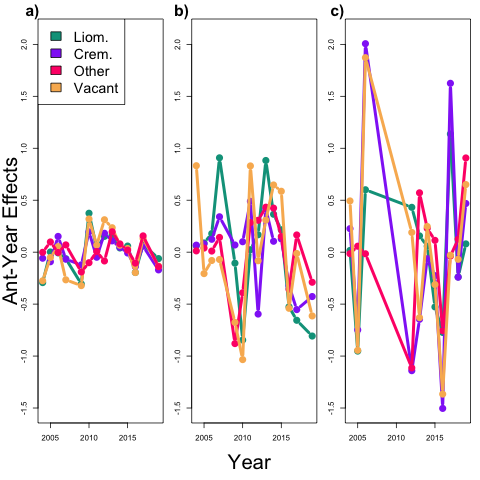
\includegraphics[width=0.58\linewidth]{year_ant_timeseries.png}
			\caption{asdasdf}
			\label{fig:year_ant}
		\end{figure}
	
		\tom{We broke down the impacts of ant partner on the growth rate by year and found that the effects of each ant on the growth rates of the cacti don’t always align, as shown in Figure \ref{fig:year-ant}. 
		In 2004, 2005, and 2007, the only ant which has a positive effect on the growth rate of the tree cholla. 
		In 2006, \textit{Crem.} has the most positive effect on the growth rate of cacti, followed by Vacant, Other, and \textit{Liom.}. 
		In 2007, 2008, and 2016, vacant had the most negative effect on the growth rates of cacti, while in 2012, vacant plants had experienced the most positive effects on their growth rates. 
		In 2010 and 2012, the only ant which has a negative effect on the growth rate of the cacti. 
		From 2013-2019, the effects of all ant partners are quite tightly coupled (all closely positive or closely negative). }{This is confusing and I think incorrect.}
		
		
		\begin{figure}[h]
			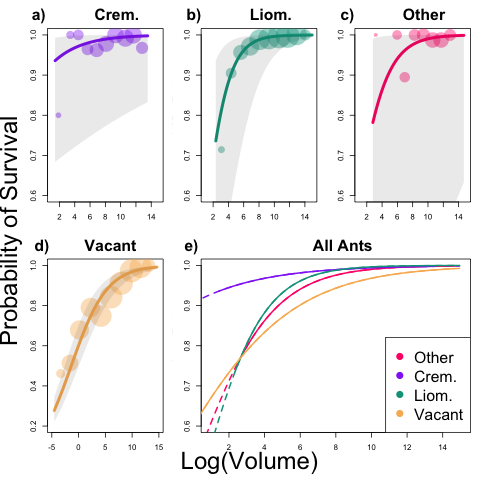
\includegraphics[width=0.58\linewidth]{surv_panels.png}
			\caption{asdasdf}
			\label{fig:surv}
		\end{figure}
		
		Our analyses of the bayesian hierarchical survival model showed that large cacti have higher survival rates than small, regardless of the ant partner. 
		It also showed that small cacti had significantly different survival rates depending on the ant partner. 
		Small cacti experienced highest survival rates when tended by \textit{Crem.} (near $70\%$) as compared to the lowest survival rates when tended by \textit{Liom.} or other ants (below $60\%$), as shown in Figure \ref{fig:surv}.
		As tree cholla grow, the probabilities of survival increase no matter the partner to nearly $100\%$ with plants tended by \textit{Crem.} and \textit{Liom.} reaching maximum survival first and plants that are vacant reaching last. 
		\textit{Crem.} tended plants have survival rates \tom{ranging}{These ranges are not meaningful because survival is so dependent on size.} from $68.379\%$ to $99.998\%$, with the rates increasing with the size of the cacti.  
		\textit{Liom.} tended plants have survival rates ranging from $35.997\%$ to $99.999\%$, with the rates increasing with the size of the cacti. 
		Other tended plants have survival rates ranging from $15.078\%$ to $99.999\%$, with the rates increasing with the size of the cacti. 
		Vacant plants have survival rates ranging from $22.031\%$ to $99.647\%$, with the rates increasing with the size of the cacti. 
		
		We broke down the survival rates by year to determine the differences in ant effects across time. 
		In 2004, 2011, 2014, and 2014, vacant tree cholla experienced more positive effects on their survival rates than any other cacti, while vacant cacti experienced the most negative effects on survival rates in 2005 and 2010.
		In 2007 and 2013, tree cholla tended by \textit{Liom.} experienced significantly more positive effects on the survival rate than any other cacti, whereas in 2018 and 2019 \textit{Liom.} tended cacti experienced the most negative effects on the survival rates. 
		In 2004 and 2009, plants tended by ants in the category of other experienced the most negative effects on survival rates, while in 2017 these plants experienced the most positive effects on the survival rates. 
		\textit{Crem.} tended tree cholla experienced more negative effects on the survival rates than any other cacti. 
		\textit{Crem.}, \textit{Liom.}, and Other-tended plants all experience similar patterns of positive and negative effects on survival rates through most years, with exceptions between the years of 2009-2010, 2011-2012, and 2017-2019. 
		
		\begin{figure}[h]
			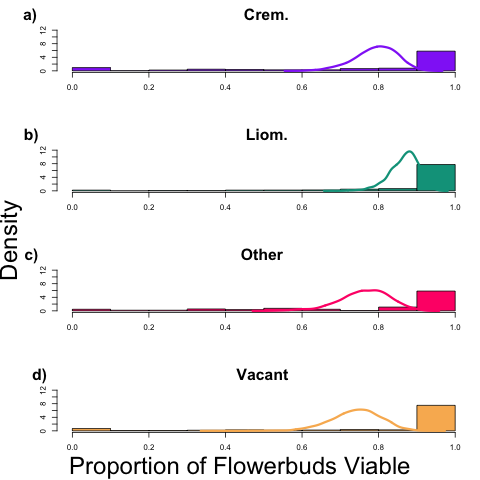
\includegraphics[width=0.58\linewidth]{Viability.png}
			\caption{asdasdf}
			\label{fig:viab}
		\end{figure}
		
		Tree cholla tended by \textit{Liom.} ants had significantly higher viability rates, from $79.83\%$ to $91.81\%$ with a mean of $87.047\%$, as compared to those of cacti tended by \textit{Crem.}, from $69.19\%$ to $87.60\%$ with a mean of $79,784\%$, and other, from $76.98\%$ to $86.20\%$ with a mean of $76.977\%$, as shown in Figure \ref{fig:viab}. 
		The lowest observed viability rate of tree cholla flower buds ranged from $62.83\%$ to $83.78\%$ with a mean of $74.604\%$ when there were no ant partners. 
		Using a \tom{chi squared test}{I did not know you did this but i don't think you should} I determined that there is a $13.6\%$ chance that this difference between the mean viability rates of \textit{Liom.} tended plants and vacant plants. 
		
		\tom{We}{I think you need to re-think these paragraphs describing the time series, because I don't think you have given readers enough info to interpret these.} broke the effects of ant partners on the viability rates of cacti down by year and found that in some years the effects of different ant partners on the viability rates of the cacti are coupled while in others they differ significantly. 
		IN 2004 vacant cacti experienced the most positive effects on their viability rates, whereas in 2005, vacant cacti experienced the most negative effects on their viability rates compared to other cacti. 
		In 2006 and 2017, \textit{Crem.} tended cacti experienced the most positive effects on viability rates, while in 2012, 2014, 2016, and 2018, \textit{Crem.} tended cacti experienced the most negative effects on viability rates. 
		In 2005,2013, 2015, and 2019, cacti tended by ants in the other category experienced the most positive effects on the viability rates, while in 2006 they experienced the most negative effects. 
		In 2012, \textit{Liom} tended cacti experienced the most positive effects on their viability rates, while in 2019 they experienced the most negative. 
		From the years 2013 to 2019, the effects of all ant partners on the viability rates of cacti are tightly coupled in patterns from positive to negative. 
		
		\subsection*{Ant Transition Rates}
			\begin{figure}[h]
			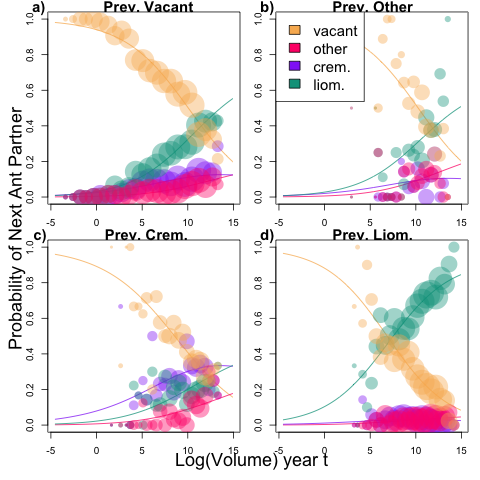
\includegraphics[width=0.58\linewidth]{Ant_Size_Multi.png}
			\caption{asdasdf}
			\label{fig:ant}
		\end{figure}
		All very small cacti \tom{are}{your tense is inconsistent} vacant with the probability of an ant partner increasing as the cacti grow larger, as shown in Figure \ref{fig:ant}. 
		Most large tree cholla are tended by \textit{Liom.} ants even if they had a different previous partner.
		The largest vacant cacti have a \tom{$42.875\%$}{we should talk about this but I don't think these point values are very effectivein the text} probability of being tended by \textit{Liom.} ants in the next season, $7.143\%$ probability of being tended by other ants in the next season, $28.571\%$ probability of being tended by \textit{Crem.}, and $21.429\%$ probability of being vacant in the next season.
		Previously vacant cacti are most likely to stay vacant until the cacti reach about $10 log(m)^3$, at which point they are more likely to be tended by \textit{Liom.} ants in the next season. 
		Large cacti tended by \textit{Liom.} ants are likely to be tended by \textit{Liom.} ants again ($90.476\%$) in the next season.
		They have a $2.372\%$ probability of being tended by \textit{Crem.} ants in the next season, $7.143\%$ probability of being tended by other ants in the next season, and $asdfasdf$ probability of being vacant.  
		Previously \textit{Liom.} tended cacti are most likely to be vacant until they reach the size of about $7 log(m^3)$, at which point they are most likely to be tended by \textit{Liom.} in the next season.
		Only large tree cholla previously tended by \textit{Crem.} are more likely to be tended by \textit{Crem.} again than be tended by \textit{Liom.} ants in the next year. 
		Large tree cholla tended by \textit{Crem.} have a $47.059\%$ probability of being tended by \textit{Crem.} in the next season, $33.333\%$ probability of being tended by \textit{Liom.} in the next season, $30\%$ probability of being tended by other ants in the next season, and $33.333\%$ probability of being vacant. 
		Previously \textit{Crem.} tended plants are most likely to become vacant in the next season until they reach the size of about $15 log(m^3)$, after which they are more likely to remain tended by \textit{Crem.} ants. 
		Cacti previously tended by other ants have a $24.138\%$ probability of being tended by \textit{Crem.} in the next season, $69.231\%$ probability of being tended by \textit{Liom.} in the next season, $7.692\%$ probability of being tended by other ants in the next season, and $23.076\%$ probability of being vacant. 
		Medium cacti follow the same patterns as large cacti in partner transitions. 
		
		\tom{}{What about the other vital rates?}
		
		\subsection*{Demographic Modeling}
		\begin{figure}[h]
			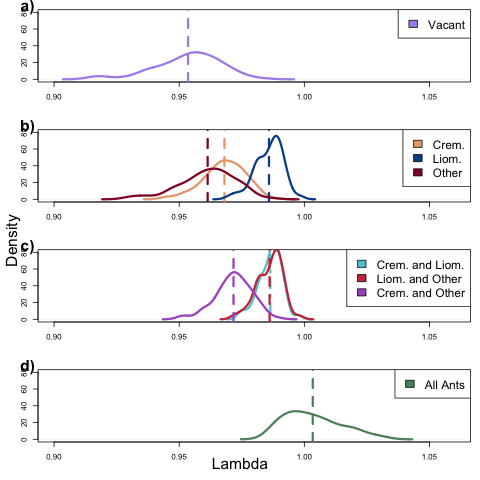
\includegraphics[width=0.58\linewidth]{lambda_det_full.png}
			\caption{asdasdf}
			\label{fig:lambda_det}
		\end{figure}
		\begin{figure}[h]
		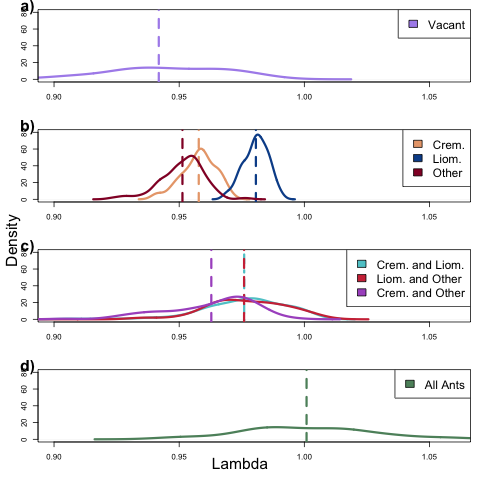
\includegraphics[width=0.58\linewidth]{lambda_st_full3.png}
		\caption{asdasdf}
		\label{fig:lambda_stoch}
	\end{figure}
		\tom{We considered both a deterministic Integral Projection Model and a stochastic one to contrast the differences.}{Just emphasizing again that the methods does not convey this.} 
		In the deterministic model, we found that \tom{simulations}{you did not provide reproducible methods for these simulations} with all ant partners (and vacancy) present resulted in the highest mean population growth rate while populations with no ant partners had the lowest mean population growth rate, as shown in Figure \ref{fig:lambda_det}.
		The estimated mean population fitness of tree cholla when all ants were present was higher than the mean population fitness of any other scenario.
		Similarly, only a few other scenarios had means within the interquartile range of this high partner diversity scenario. 
		\tom{Honestly have no idea how much detail I should go into in this? }{It's less a matter of detail (though more would be good) and more about having a point. Your text seems to describe the results in a quasi-random, surface-level way. Bring more intention to your decisions about what to write here. What does a reader need to know to understand the story you are trying to tell?}
		
		
		\section*{Discussion}
		\tom{\subsection*{Vital Rates}}{I don't think these are the right subsection headings because they are simply redescribing results.}
		\textbf{Ant partners have contrasting effects on vital rate processes of tree cholla.}
		Regression analyses showed that the different ant partners had significantly different impacts on the various vital rate processes of the tree cholla cacti. 
		Specifically, \textit{Crem.} tended cacti have advantages, at small sizes, over cacti tended by any other ant or vacant. 
		\textit{Crem.} tended tree cholla had the highest survival rates (Figure \ref{fig:surv})  at small sizes and the highest growth rates (Figure \ref{fig:grow}), two of the most important vital rates for small cacti which are not yet reproducing. 
		On the other hand, reproducing cacti which have \textit{Liom.} partners  have advantages with the highest viability rates of flower buds (Figure \ref{fig:viab}). 
		Together this indicates that the best partner may change as the cacti grow and begin to reproduce, when the most vulnerable part of the plant is the flower with the seeds. 
		This reflects the changes in the resource use of tree cholla as they begin to use their resources for reproduction rather than growth. 
		The fact that different ant partners have significantly different effects on the various vital rates of tree cholla indicates that none of them are the “perfect” partner, and that the “best” partner may in fact change over the lifespan of the cacti. 
		As the tree cholla grew, the best partner changed from \textit{Crem.} ants, partners known for ***, to \textit{Liom.} ants, partners best known for defensive benefits to the cacti, particularly against the seed predators which most impact viability. 
		The difference in ant partners made a significant difference in the observed vital rates of the cacti, indicating that \tom{considering the interaction between the tree cholla and any individual partner would fail to capture the extent of the benefits}{great point and well made -- I am going to stop commenting on the rest of the discussion because I think it needs to be re-worked. We can discuss more.} to the cacti.
		Like many other systems, pairwise perspectives do not fully encompass the complex impacts that multispecies mutualisms have on the focal mutualists vital rates.
		
		\subsection*{Ant Transition Rates}
		\textbf{Small cacti remain vacant, while large cacti are most likely to be tended by \textit{Liom.} ants.}
		Small cacti are unlikely to be tended because most do not produce EFN, of if they do it is a very small amount. 
		Medium-sized to large cacti are much more likely to be tended than vacant as they begin producing EFN, with many factors that determine the most likely partner. 
		Some of the ant partners appear to have high turnover rates, meaning they are unlikely to tend the same plant multiple years in a row. 
		Ants in the other category have high turnover rates, shown by the fact that medium and large cacti tended by other are unlikely to be tended by other ants again in the next season. 
		The reason for these turnovers could be due to the inability to defend their territories, an ability to find and colonize new resources, or an ability to colonize resources that have been left unclaimed. 
		This discovery-dominancy tradeoff is a well-studied hypothesis in ant literature \cite{lach2010} that could explain the remaining presence of ants in the other category despite high turnover rates.
		
		
		On the other hand, \textit{Crem.} ants appear to have lower turnover rates, since large cacti have up to $47.059\%$ probability of being tended by \textit{Crem.} in the next year.
		In addition to turnover rates, there are also colonization rates, the probability of a species taking over a cactus that was previously tended by different ants. 
		\textit{Liom.} are the only ant partners we observed with high colonization rates. 
		Most cacti tended by non-\textit{Liom.} ants have a high probability of being taken over by \textit{Liom} ants in the next season, as shown in Figure \ref{fig:ant}.
		This pattern could be due to the well-known high levels of aggression displayed by \textit{Liom.} ants in this system, however there are other possible explanations, such as nectar composition.
		The exception to this rule are plants tended by \textit{Crem.} ants which are more likely to remain tended by \textit{Crem.} than be taken over by \textit{Liom.} in the next season. 
		The trend that most large ants are likely to be tended by \textit{Liom.} ants reflects the findings that large cacti benefit most from \textit{Liom.} as ant partners. 
		As explained in the introduction, there are many factors that determine the colonization rates of different cacti by their ant partners, including EFN quantity and quality, ability to seek out cacti, aggression, and more.
		These patterns could be explained by the \textit{Liom.} ants ability to dominate at a resource site and therefore takeover from different ants which originally found the site. 
		
		
		An alternative, or parallel, explanation for these ant transitions could be the changes in EFN composition across ontogeny of the cacti.
		As cacti grow the chemistry of EFN produced changes ***, changing from more *** composition to *** composition. 
		Different ants have preferences for different nectar compositions\cite{Lach2010}, specifically, ***.
		This could provide a potential route for the cacti to select their own ideal partners
		This indicates a potential future avenue of research into the correlations between ant partners and the chemistry of the EFN produced by the tree cholla. 
		
		\subsection*{Demographic Modeling}

	
\end{document}

\typeout{\bibliography{References.bib}}
